\RequirePackage{lineno}
\documentclass{revtex4}
%\usepackage[pdftex]{graphicx}

\usepackage{amsmath,amsfonts,amssymb}
\usepackage[english]{babel}
\usepackage[latin1]{inputenc}
\usepackage[T1]{fontenc}
\usepackage{color}
\usepackage{float}
\usepackage{verbatim}
\usepackage{graphicx}
\usepackage{bm}
\usepackage{mathtools}
\usepackage{stmaryrd}
\usepackage{anyfontsize}

\usepackage[font={small}]{caption}
\usepackage{subcaption}
\captionsetup{compatibility=false}
\usepackage{xr}
\externaldocument[extfig-]{msv6}
%\usepackage{epstopdf}
%\usepackage{array}
%\usepackage{tabularx}
%\usepackage{multirow}
\usepackage{color}
%\usepackage{multibox}
%\usepackage{rotating}
% \usepackage{lineno}

%\usepackage[left]{lineno}
%\usepackage[comma,sort&compress]{natbib}
%\usepackage{authblk}
%\usepackage{multicol}

\linespread{1.5}

\usepackage{natbib}
\bibpunct{(}{)}{,}{a}{}{;}

% \bibliographystyle{prsb}

% \usepackage{bibunits}

\newcommand{\beginsupplement}{%
        \clearpage
        \setcounter{table}{0}
        \renewcommand{\thetable}{S\arabic{table}}%
        \setcounter{figure}{0}
        \renewcommand{\thefigure}{S\arabic{figure}}%
     }

% \pagewiselinenumbers
\linenumbers
% \setlength\linenumbersep{3pt}

\begin{document}

% \Blindtext
%\title{Simple rules yield complex communities: deconstructed species interactions and the assembly of communities}
%\title{Community assembly and dynamics by the deconstruction of species interactions}
\title{Supplementary Figures: Eco-evolutionary dynamics and collective dispersal: implications for salmon metapopulation robustness}
\author{
Justin D. Yeakel${}^{1,2,*}$, Jean P. Gibert${}^{1}$, Peter A. H. Westley${}^{3}$, \& Jonathan W. Moore${}^{4}$ \\
${}^1$School of Natural Sciences, University of California, Merced, Merced CA, USA \\
${}^2$The Santa Fe Institute, Santa Fe NM, USA \\
${}^3$College of Fisheries and Ocean Sciences, University of Alaska, Fairbanks, Fairbanks AK, USA \\
${}^4$Earth${}_2$Oceans Research Group, Simon Fraser University, Vancouver BC, Canada \\
${}^*$To whom correspondence should be addressed: jdyeakel@gmail.com
}

\maketitle

\beginsupplement

\section*{I. Gaussian approximation for the mixed trait distribution}
We assume a Gaussian distribution to approximate the more complex trait distribution that results when two populations with two distinct trait distributions are linked by gene flow and reproduction.
Here and throughout, we refer to the resident population as $i$ and the straying population as $j$, though both populations stray simultaneously.
The Gaussian approximation is assumed to have a mean that is equal to the mean of the mixed trait distribution $(1-m)\mu_i + m\mu_j$ with a constant variance $\sigma^2$, equal to the original trait variance prior to mixing.
We employ this approximation because a mixed trait distribution that remixes and recombines (through reproduction) at each time-step becomes complicated very quickly, as we shall demonstrate.
\emph{Importantly, because the evolutionary framework tracks only the mean and not the variability through time, this approximation is exact with respect to the first moment.}
Accordingly, the only attribute that is approximate is the assumption of normality.
Below we will show that a constant variance of $\sigma^2$ for the mixed trait distribution is a good approximation in most relevant cases, and becomes increasingly accurate when 1) generations become less overlapping (i.e. the case of semelparity), and 2) with density-dependent straying ratios.


{\bf The trait distribution at $\bm{t=0}$.} At time $t=0$, it is assumed that individuals from two separate populations have not yet mixed. 
Thus, the mean trait values for both populations are equal to the optimal trait values that accord to their respective habitats $\mu_i(t=0) = \theta_i$, and that their trait values are distributed as $X_i=x_i \sim g(x_i,\mu_i,\sigma) = \mathcal{N}(\mu_i,\sigma)$.
Here and henceforth we use upper-case to denote random variables, and lower-case to denote specific values of random variables.

{\bf The trait distribution at $\bm{t=1}$.} At time $t=1$, dispersal of individuals from site $j$ to site $i$, and vice versa, has begun.
The proportion of individuals that disperse to and from each population is given by the stray ratio $m$.
The calculation of the mixed distribution that results from dispersal and subsequent recruitment incorporates the following processes:
\emph{1)} dispersal of strays into the local population from the remote population, and vice versa;
\emph{2)} recruitment of juveniles that are produced from this mixed distribution (under the assumption of random mating); 
\emph{3)} mortality of individuals in the adult class.
These events occur in the order in which they are listed.

The mixed trait distribution for site $i$ immediately following dispersal is simply a mixed Gaussian with weights determined by the proportion of the population that are residents $i$ and the proportion that are strays $j$, such that 
\begin{equation}
  p(x_{\rm disperse}) = w_i g(x_i,\mu_i,\sigma) + (1-w_i)g(x_j,\mu_j,\sigma),
\end{equation}
where the proportion of the population $i$ composed of \emph{resident} individuals is
\begin{equation}
  w_i = \frac{(1-m)N_i}{(1-m)N_i + mN_j},
\end{equation}
and the proportion of population $i$ composed of strays is $(1-w_i)$.
Once individuals in both habitats mix, they mate without preference.
Recruits are assumed to have trait values intermediate to their parents such that $x_{\rm r} = (x_{1} + x_{2})/2$ where trait values $X_1=x_{1}\sim p(x_{\rm disperse})$ and $X_2=x_{2}\sim p(x_{\rm disperse})$.
We thus assume that parental traits are drawn independently from the mixed distribution $p(x_{\rm disperse})$, conditional on the requirement that $x_2 = 2x_r - x_1$, which we get when rearranging the equation for $x_{\rm r}$.
Incorporating this condition and that traits are independently drawn from the mix of residents and strays yields the probability density for the trait value of recruits,
\begin{equation}
  q(x_{\rm r}) = \int_{-\infty}^\infty 2p(x_1)p(2x_{\rm r}-x_1){\rm d}x_1,
\end{equation}
where the factor of 2 comes from...
The mean of the recruit trait distribution is calculated to be
\begin{equation}
{\rm E}\{q(x_{\rm r})\}=(1-m)\mu_i + m\mu_j,
\end{equation} 
and the variance is
\begin{equation}
  {\rm Var}\{q(x_{\rm r})\} = \frac{m^2 N_j^2 \left(4 \mu_j^2+\sigma ^2\right)+(m-1)^2 N_i^2 \left(4 \mu_i^2+\sigma ^2\right)-(m-1) m N_i N_j \left(\mu_i^2+6 \mu_i \mu_j+\mu_j^2+2 \sigma ^2\right)}{2 (-m N_i+m N_j+N_i)^2}.
\end{equation}

The relative contribution of trait values from resident parents, stray parents, and recruits depends on the numbers of each within the mixed population.
The number if residents is $(1-m)N_i$, and the number of strays is $mN_j$.
However, because adult mortality occurs after reproduction, we must adjust these numbers to account for only those who survive, which is given by ${\rm e}^{-Z}$.
As $Z\rightarrow \infty$, the population becomes semelparous, as the adult class gives way to new recruits at each timestep. 
Accordingly, the number of adult residents and strays is given by $(1-m)N_i{\rm e}^{-Z}$ and  $mN_i{\rm e}^{-Z}$, respectively.
In contrast, the number of recruits is given by the combined contribution of resident and straying individuals to recruit production as $N_r = ((1-m)N_1 R[\mu_i] + mN_2 R[\mu_j]){\rm e}^{(-\beta((1-m)N_i + mN_j))}$ where $R$ is the recruitment rate, which differs for resident vs. straying individuals (see manuscript, Eq 2).

\begin{figure}
  \captionsetup{justification=raggedright,
singlelinecheck=false
}
\centering
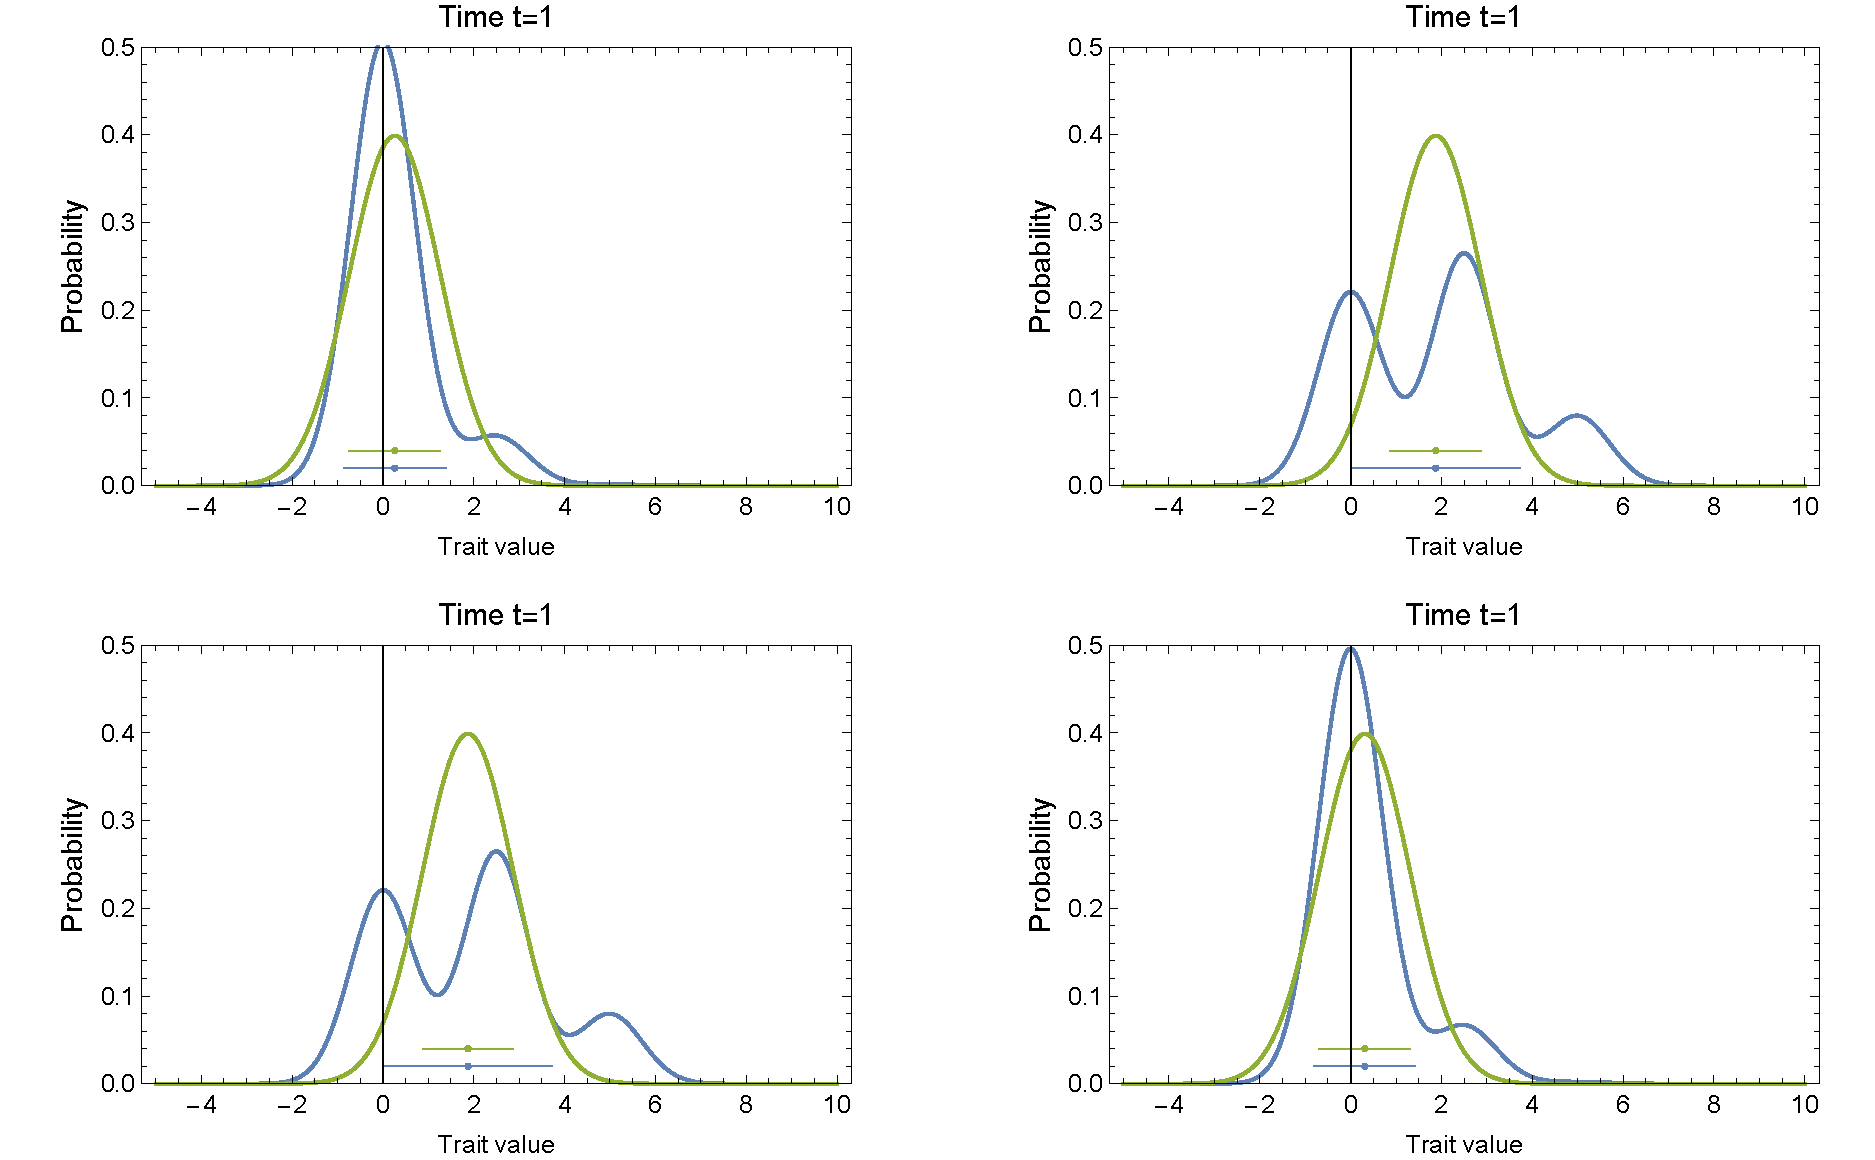
\includegraphics[width=0.7\textwidth]{fig_PDF.pdf}
\caption{
Clockwise from the upper-left. The calculated probability distribution function (PDF) for individuals in population $i$ after immigration from population $j$, recruitment, and mortality (blue) vs. the Gaussian approximation used for the dynamical system (green), with
a) low stray ratio, large straying population, overlapping generations: $m=0.1$, $Z=0.5$;
b) high stray ratio, overlapping generations: $m=0.5$, $Z=0.5$;
c) high stray ratio, non-overlapping generations: $m=0.5$, $Z=1000$;
d) density-dependent stray ratio, non-overlapping generations: $m=m_0(1-N_i/(C+N_i))$, $Z=1000$, where $m_0=0.2$ and $C=1000$.
The mean and variability of both distributions is shown by a point (mean) and line ($\sigma$) at the base of each distribution.
} \label{fig:PDF}
\end{figure}



The proportion of individuals from the resident, straying, and recruitment classes following mortality at site $i$ are then $c_i$, $c_j$, and $c_r$ respectively, where
\begin{align}
c_i &= \frac{(1-m)N_i{\rm e}^{-Z}}{(1-m)N_i{\rm e}^{-Z} + m N_j{\rm e}^{-Z} + N_r} \\ \nonumber
c_j &= \frac{m N_j{\rm e}^{-Z}}{(1-m)N_i{\rm e}^{-Z} + m N_j{\rm e}^{-Z} + N_r} \\ \nonumber
c_r &= \frac{N_r}{(1-m)N_i{\rm e}^{-Z} + m N_j{\rm e}^{-Z} + N_r}.
\end{align}
where $c_i + c_j + c_r= 1$.
The trait value distribution for time $t=1$ is then calculated as a mix of trait distributions from 1) surviving residents, 2) surviving strays, and 3) their offspring, such that
\begin{equation}
  g_{{\rm next}}(x_i) = c_i g(x_i) + c_j g(x_j) + c_r q(x_r).
\end{equation}
The expectation of this distribution is
\begin{equation}
{\rm E}\{g_{\rm next}(x_i)\}=(1-m)\mu_i + m\mu_j,
\end{equation} and the variance is
% variance a that has a closed form solution, but that is not easily readable.
\begin{align}
  {\rm Var}\{g_{{\rm next}}(x_i)\}=&\frac{(\mu_i-\mu_j)^2 (2 (m-1)^2 N_i^2 c_j^2-(m-1) N_i c_j (2 (m-1) N_i+m N_j (1-4 c_i))}{2 (-m N_i+m N_j+N_i)^2} \\ \nonumber
  &+ \frac{m N_j (c_i-1) (-m N_i+2 m N_j c_i+N_i))-\sigma ^2 (c_i+c_j+1) (-m N_i+m N_j+N_i)^2}{2 (-m N_i+m N_j+N_i)^2}.
\end{align}

Importantly, ${\rm E}\{g_{{\rm next}}(x_i)\}$ is exactly equal to the trait mean for the original mix, as well as the trait mean for recruits.
Thus, a Gaussian approximation distributed as $\mathcal{N}(w_i\mu_i + (1-w_i)\mu_j,\sigma)$ will not alter the dynamics under the assumption of constant variance in Eq 4.
Moreover, the mixed distribution described above becomes more complex at the next timestep, as two multi-modal trait distributions then mix and recombine through recruitment.
Although the complexity of the true distribution is increased and becomes quickly intractable, one expects the actual form to eventually approximate a Gaussian based on the central limit theorem.
One could make the argument that a Gaussian approximation does not represent the multi-modality in trait values inherent to a mixed distribution, and thus underestimates variance.
Although the Gaussian approximation exactly captures the expectation, we next explore to what extent the approximation does and does not capture the variability expressed in $g(x_{\rm next})$.

%Discussion of factors that increase or decrease accuracy of the approximation
The Gaussian approximation $\mathcal{N}(w_i\mu_i + (1-w_i)\mu_j,\sigma)$ will generally underestimate the true variance of the mix, but not by much.
If the straying ratio is low, (ca. 0.0 to 0.2), the Gaussian approximation tends to be very similar to the actual distribution (Fig. \ref{fig:PDF}a).
As the straying ratio increases, so does the bimodality of the actual distribution, and this magnifies our underestimate of variance (Fig. \ref{fig:PDF}b).
The interesting dynamics observed in our model generally occur between $m=0.05$ and $m=0.2$, where estimates of variance are similar.
Decreasing the overlap between generations also leads to greater similarity in the actual distribution and the Gaussian approximation, and the potential bias introduced by bimodality will be less for cases of non-overlapping generations, or semelparity (Fig. \ref{fig:PDF}c).
Most importantly, density-dependent straying increases the accuracy of our Gaussian approximation by suppressing the straying ratio (Fig. \ref{fig:PDF}d).

Because the Gaussian approximation is exact to first order, and generally provides a good approximation of realized variance, we suggest that the use of Lande's formulation for the change in mean trait values through time under the assumption of constant variance is appropriate (see Eq. 4 in main text).
Because our estimate of variance is generally an underestimate, the rate of recruitment will be a slight overestimate (Eq. 2, main text), and the timescale of trait evolution will generally be slower (Eq. 4, main text).
Changes in the rate of recruitment (Fig. \ref{fig:symmetry}) and heritability do not have an impact on our qualitative findings, and this suggests any bias that our approximation introduces by underestimating true variance is minimal.




\section*{II. Additional Figures}


% \begin{figure}
%   \captionsetup{justification=raggedright,
% singlelinecheck=false
% }
% \centering
% 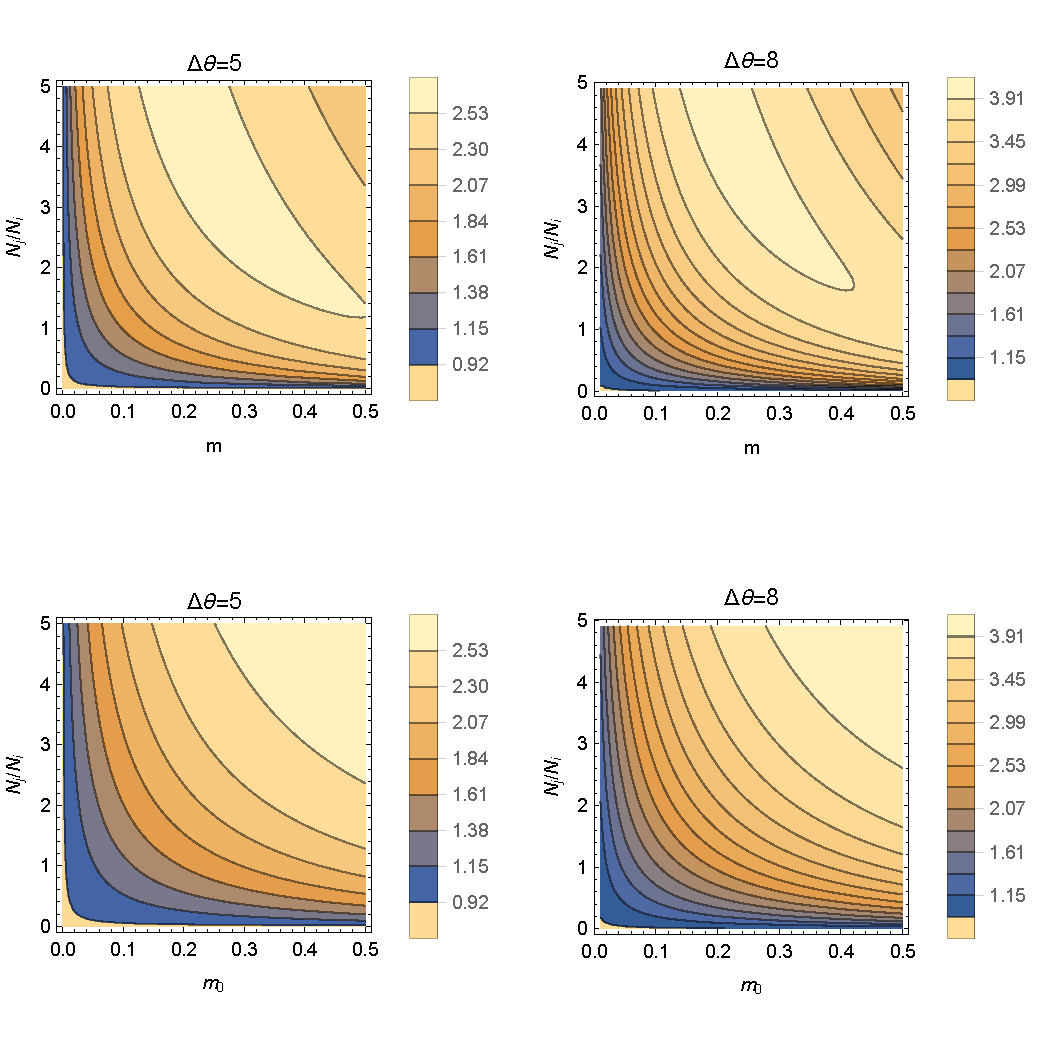
\includegraphics[width=0.7\textwidth]{fig_contSD.pdf}
% \caption{
% Magnitude of difference in the standard deviation for the calculated PDF for individuals in population $i$ after 1) immigration from population $j$, 2) recruitment, and 3) adult mortality vs. the Gaussian approximation where $\sigma=1$.
% Values $<1$ reflect underestimates of variability; values $>1$ reflect overestimates.
% Top row is for constant straying ratio, and the bottom row is for density-dependent straying ratio under different treatments of habitat heterogeneity (left column $\Delta \theta=5$; right column $(\Delta \theta=8$).
% } \label{fig:contourSD}
% \end{figure}
% 




\begin{figure}
  \captionsetup{justification=raggedright,
singlelinecheck=false
}
\centering
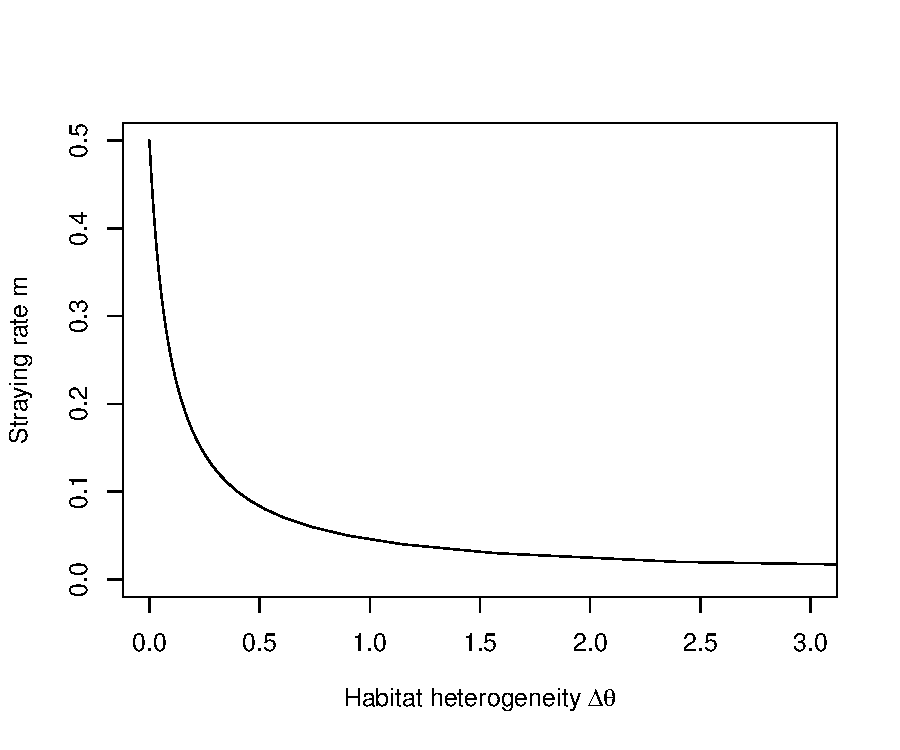
\includegraphics[width=0.35\textwidth]{fig_mthetarelation.pdf}
\caption{
In some cases, habitat heterogeneity may be assumed to determine the rate of straying, if for example:
1) sites are distributed over greater spatial distances, where habitat differences are assumed to be greater between more distant sites, or 2) individuals have behaviors promoting dispersal between habitats that are more similar. To examine such cases, we use the relationship $m= 0.5(1 + \Delta\theta)^{-1}$ where maximum straying is assumed to occur at $m=0.5$ (perfect mixing).
} \label{fig:mthetarelation}
\end{figure}


\begin{figure}
  \captionsetup{justification=raggedright,
singlelinecheck=false
}
\centering
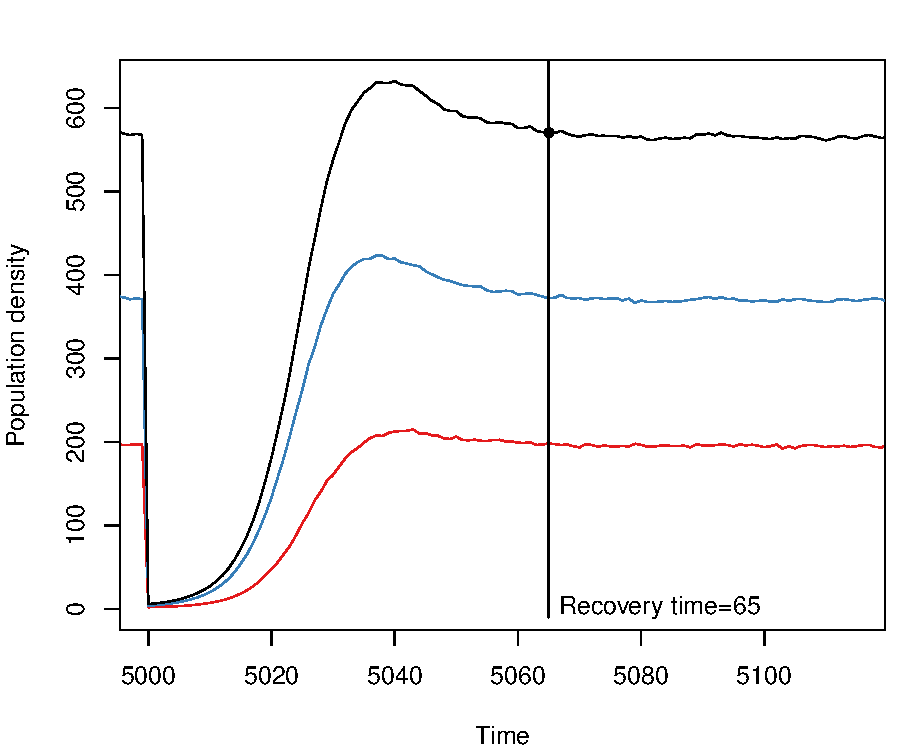
\includegraphics[width=0.35\textwidth]{fig_recovery.pdf}
\caption{
Example of the numerical procedure used to estimate recovery time. After a disturbance is introduced, the recovery time is calculated by measuring the point in time where $N_T$ (in black), which is the aggregate of both populations (blue, red) settles to within one standard deviation of the new equilibrium $N_T^*$. 
} \label{fig:recovery}
\end{figure}


\begin{figure}
  \captionsetup{justification=raggedright,
singlelinecheck=false
}
\centering
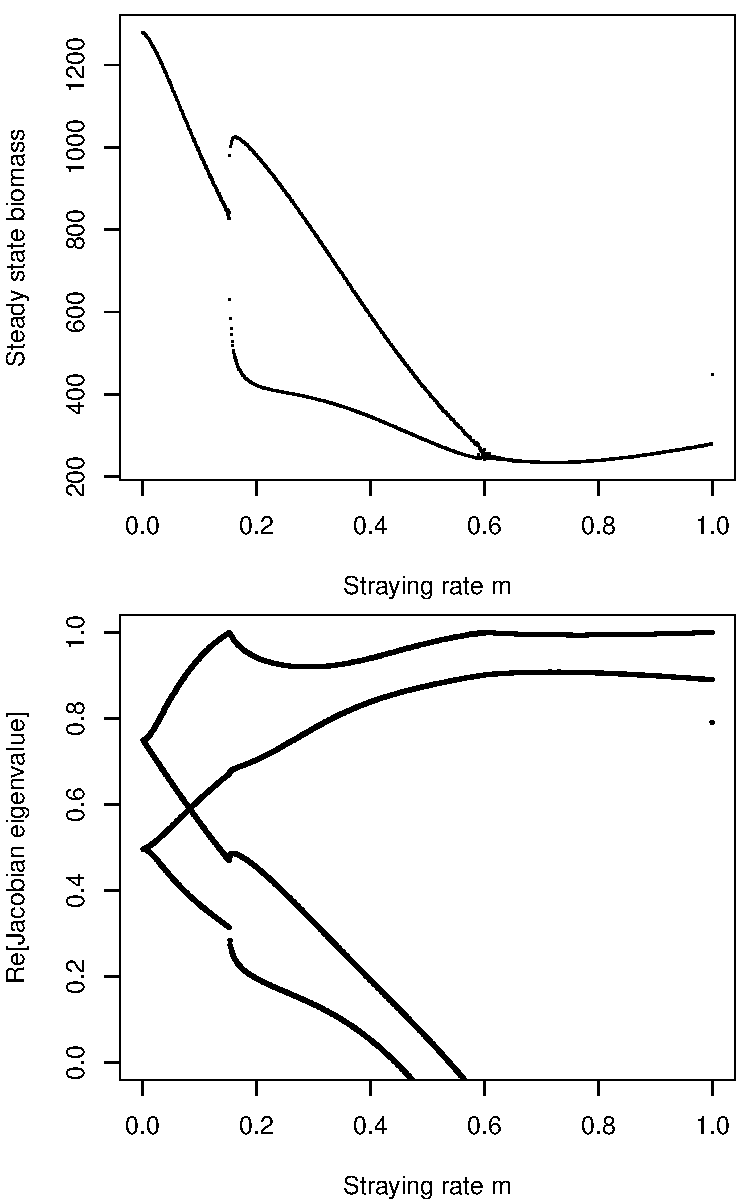
\includegraphics[width=0.35\textwidth]{fig_eigs.pdf}
\caption{
The real parts of the four eigenvalues for the Jacobian matrix of the 4-dimensional system.
The cusp bifurcation occurs when the dominant eigenvalue crosses the unit circle at $+1$. 
} \label{fig:eigs}
\end{figure}


\begin{figure}
  \captionsetup{justification=raggedright,
singlelinecheck=false
}
\centering
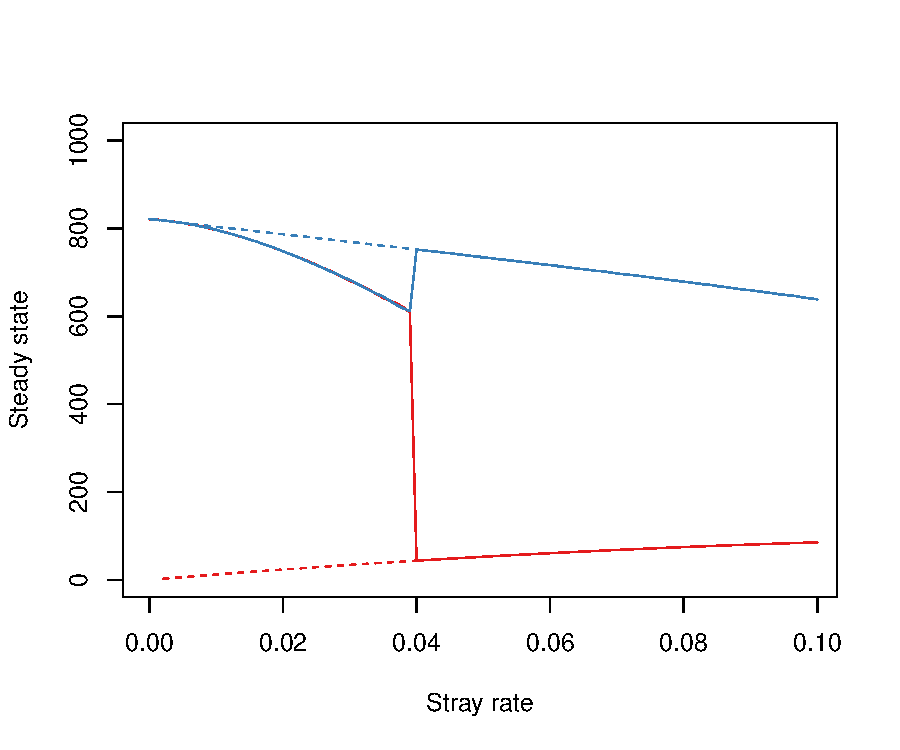
\includegraphics[width=0.35\textwidth]{fig_hysteresis.pdf}
\caption{
Increasing the straying rate results in the transition from a single steady-state for both populations to a dominant and subordinate states. If the straying rate is subsequently lowered, the single steady-state is not easily obtained, which is the hallmark of hysteresis.
} \label{fig:hysteresis}
\end{figure}




\begin{figure}
  \captionsetup{justification=raggedright,
singlelinecheck=false
}
\centering
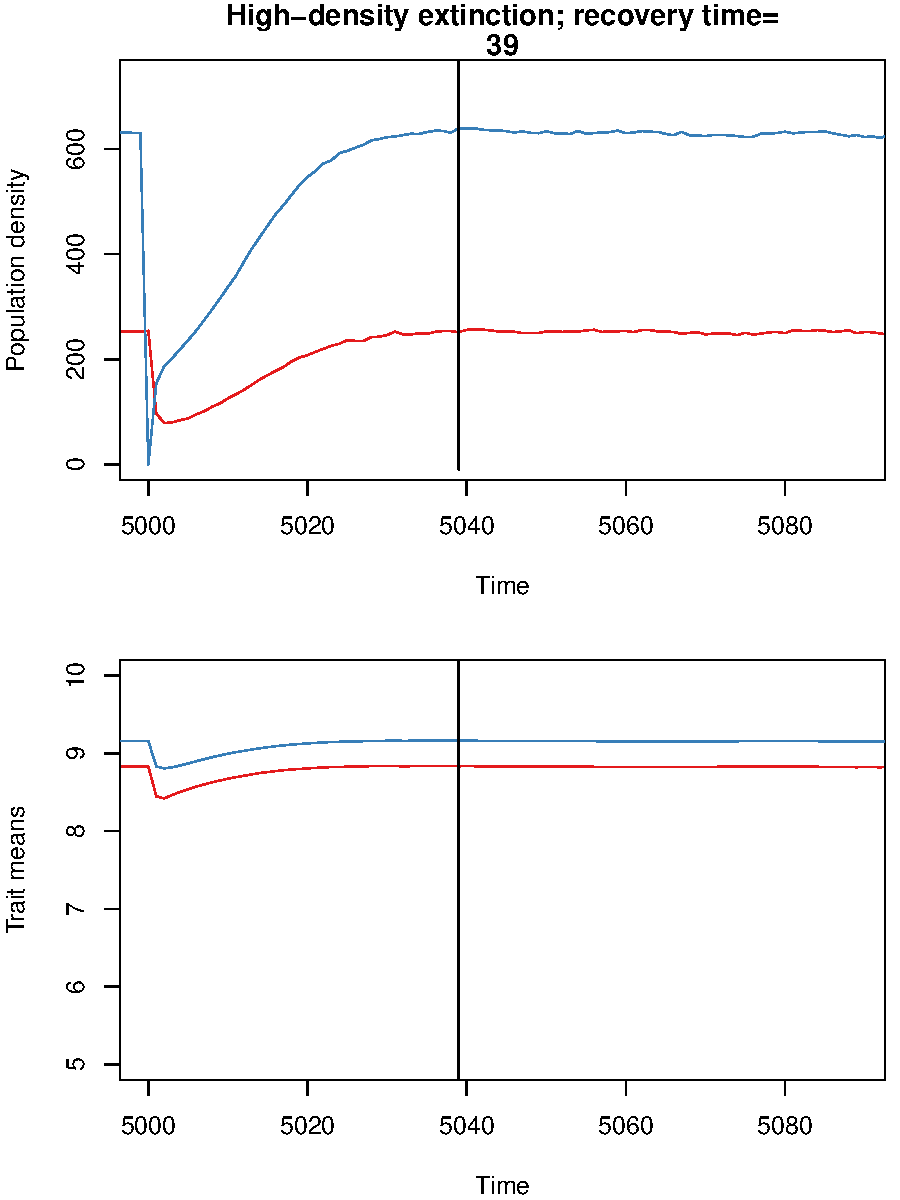
\includegraphics[width=0.35\textwidth]{fig_relax_large.pdf}
\caption{
Extinction of high-density population with a high straying rate $m=0.4$ and low trait heritability $h^2=0.2$ (see figure \ref{extfig-fig:relax}a).
Black line marks the calculated point of recovery post-perturbation.
Trait optima are $\theta_1 = 10$ (blue population trajectory) and $\theta_2 = 5$ (red population).
} \label{fig:relaxtraj_hdlh}
\end{figure}


\begin{figure}
  \captionsetup{justification=raggedright,
singlelinecheck=false
}
\centering
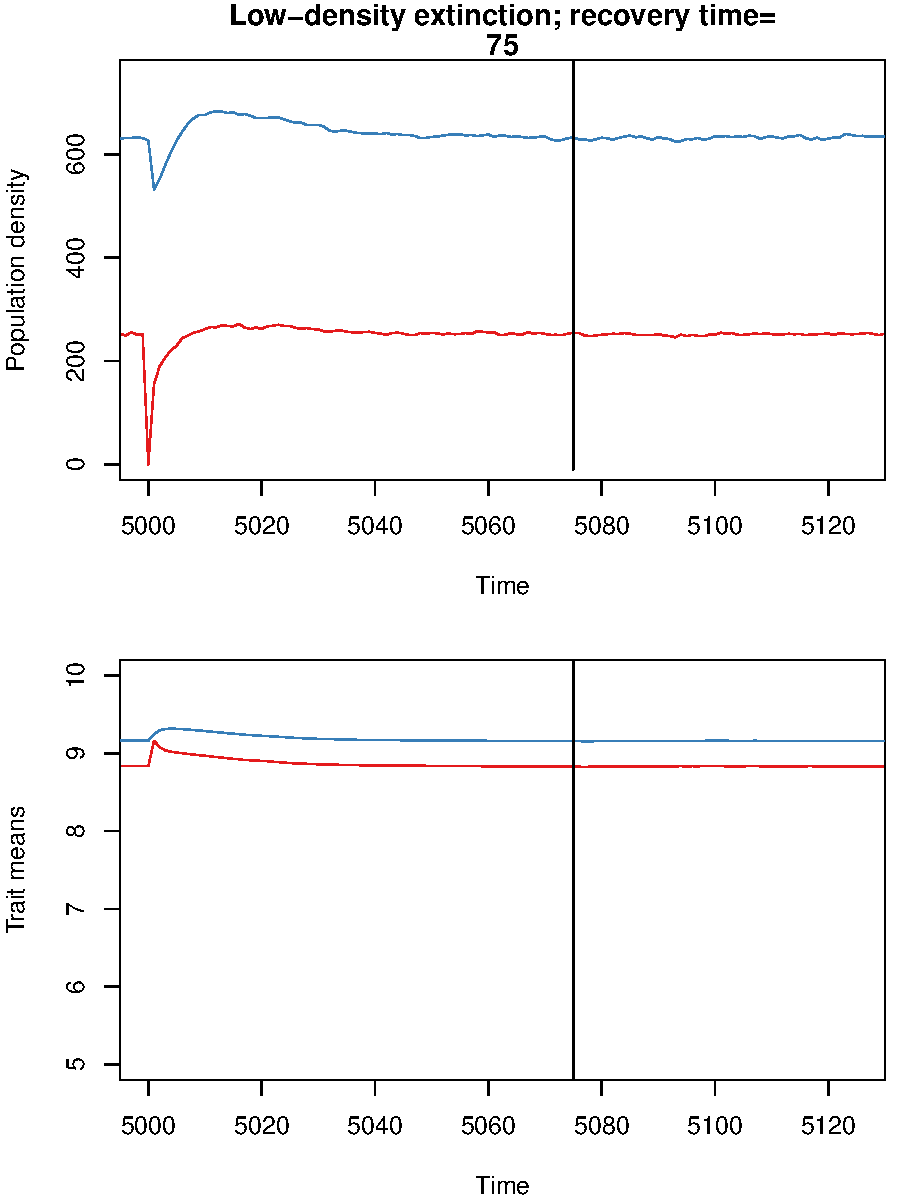
\includegraphics[width=0.35\textwidth]{fig_relax_small.pdf}
\caption{
Extinction of low-density population with a high constant straying rate $m=0.4$ and low trait heritability $h^2=0.2$ (see figure \ref{extfig-fig:relax}a).
Black line marks the calculated point of recovery post-perturbation.
Trait optima are $\theta_1 = 10$ (blue population trajectory) and $\theta_2 = 5$ (red population).
} \label{fig:relaxtraj_ldlh}
\end{figure}



\begin{figure}
  \captionsetup{justification=raggedright,
singlelinecheck=false
}
\centering
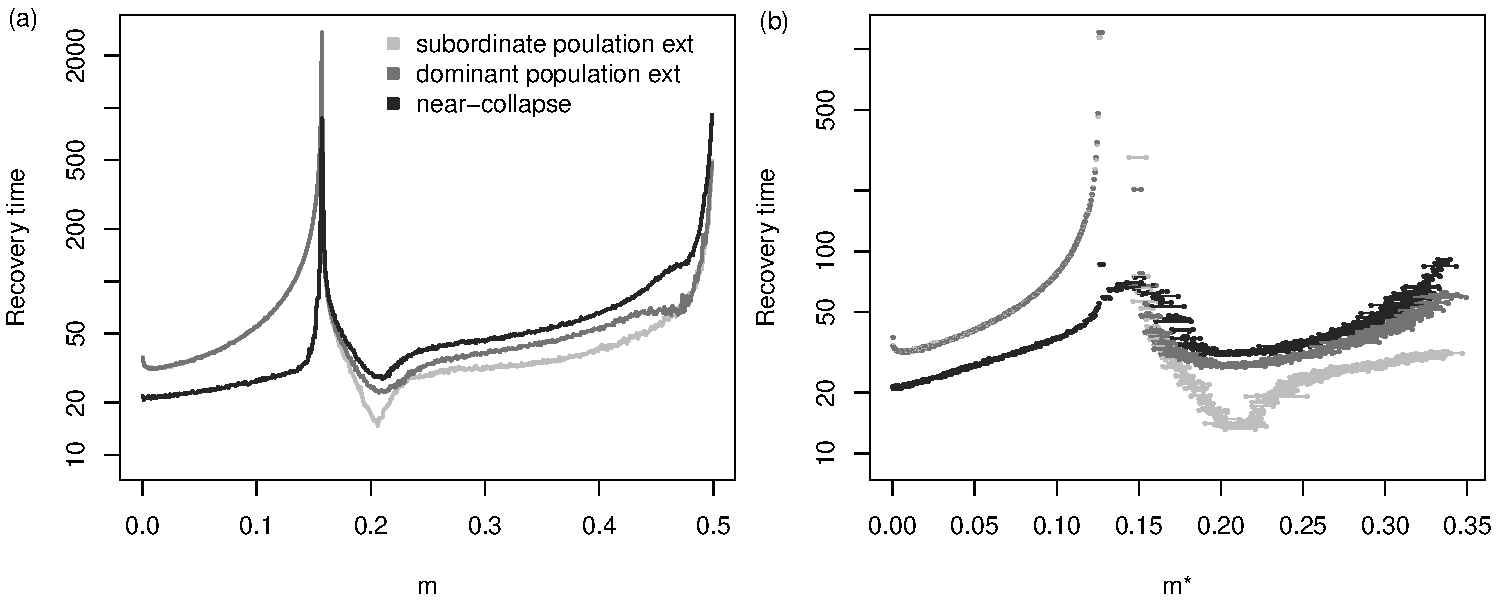
\includegraphics[width=0.9\textwidth]{fig_relax_highh.pdf}
\caption{
Recovery time of $N_T$ following the extinction of either the low-density (light gray) or high-density (gray) population, or the near-collapse of both (dark gray) assuming (a) constant straying rates $m$ and (b) density-dependent straying rates (evaluated at the steady-state $m^*$) with trait heritability $h^2=0.8$.
If $m$ is density-dependent, in the alternative stable state regime there are two straying rates observed: one each for the low- and high-density populations, respectively, which are linked by a horizontal line.
} \label{fig:relax_highh}
\end{figure}



\begin{figure}
  \captionsetup{justification=raggedright,
singlelinecheck=false
}
\centering
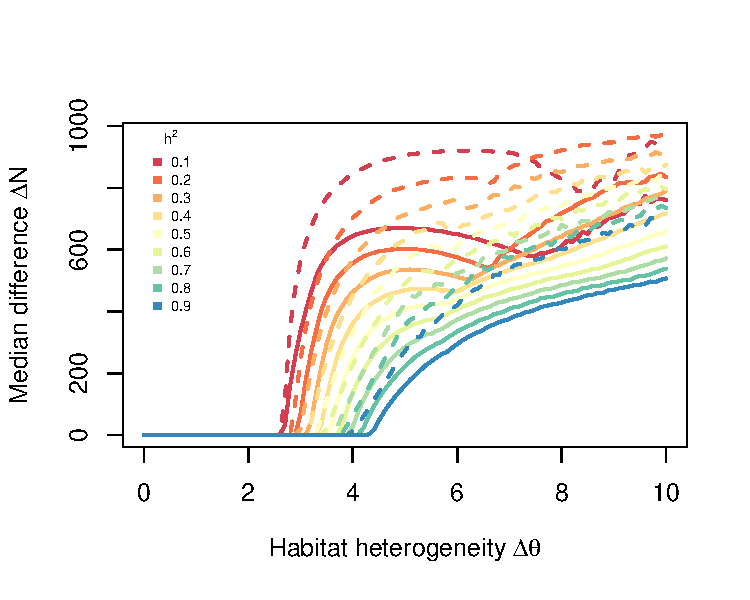
\includegraphics[width=0.4\textwidth]{fig_thetadiffN.pdf}
\caption{
Median difference in population densities taken over the straying rate as a function of habitat heterogeneity $\Delta\theta$.
Solid lines are for constant $m$; dashed lines are for density-dependent $m$.} \label{fig:thetadiffN}
\end{figure}


\begin{figure}
  \captionsetup{justification=raggedright,
singlelinecheck=false
}
\centering
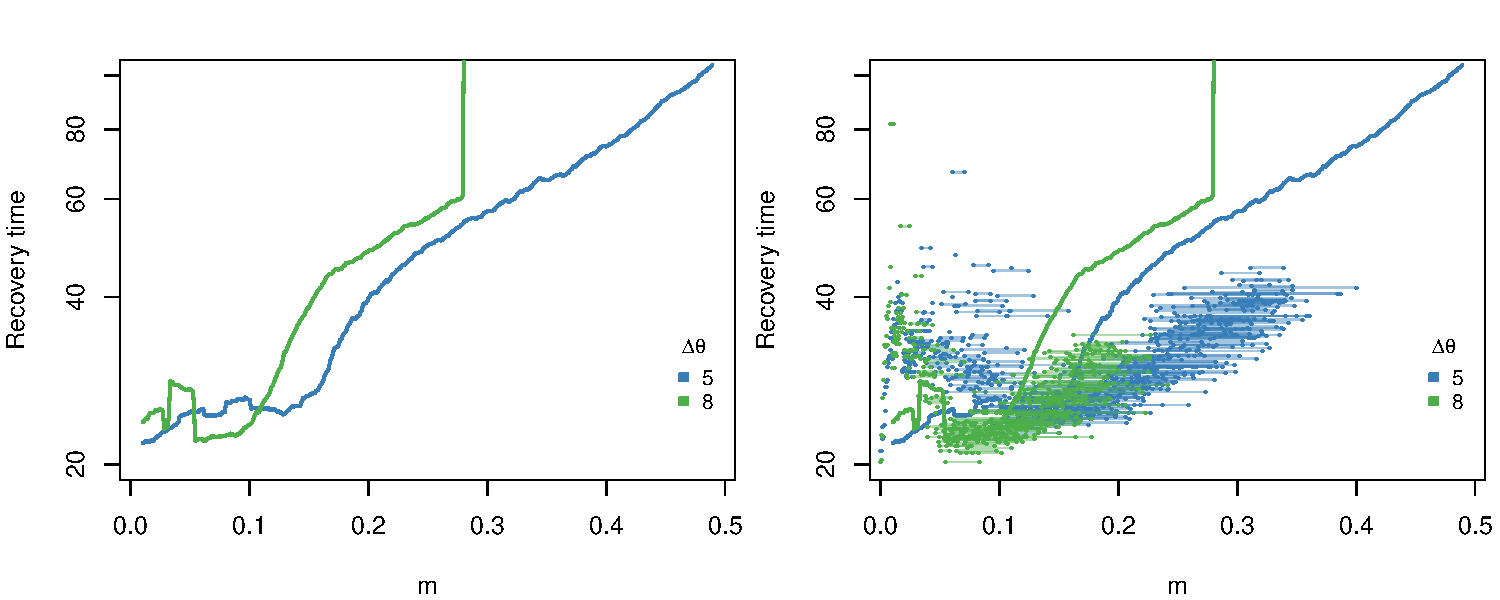
\includegraphics[width=0.8\textwidth]{fig_relaxtheta2.pdf}
\caption{
(a) Recovery time after near collapse of both populations as a function of straying rate $m$ and habitat heterogeneity $\Delta\theta$.
(b) The same as (a) but including recovery times when straying is density-dependent evaluated at $m^*$, shown by linked point pairs.
Recovery times for systems with density-dependent straying are longer when straying is low and shorter when straying is high, mirroring the change in portfolio effects with respect to density-dependent straying shown in figure \ref{extfig-fig:thetaPE}.
} \label{fig:relaxtheta}
\end{figure}



\begin{figure}
  \captionsetup{justification=raggedright,
singlelinecheck=false
}
  \centering
  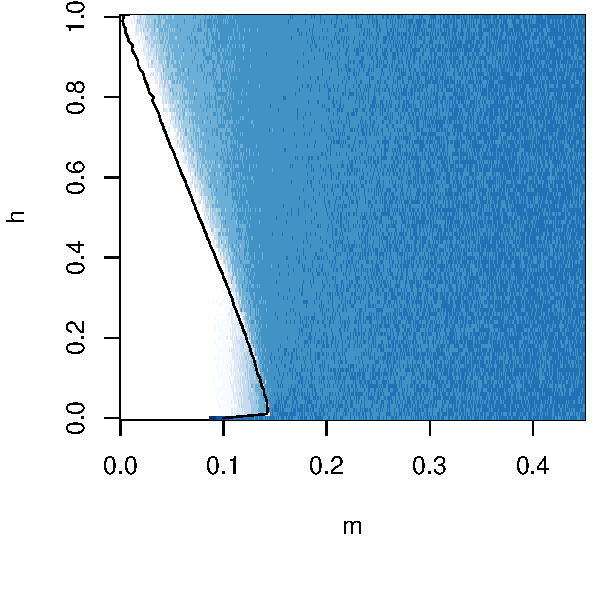
\includegraphics[width=0.35\textwidth]{fig_MDPE_hm_mtheta_rt.pdf}
  \caption{
  Portfolio effects as a function of straying rate $m$ and trait heritability $h^2$ when the rate of straying is $m = 0.5(1 + \Delta\theta)^{-1}$. Alternative steady-states emerge for low values of $m$ (left of the cusp bifurcation, denoted by the black line), whereas a single steady-state exists for high $m$.
  } \label{fig:mthetaPE}
\end{figure}

% \clearpage

\begin{figure}
  \captionsetup{justification=raggedright,
singlelinecheck=false
}
\centering
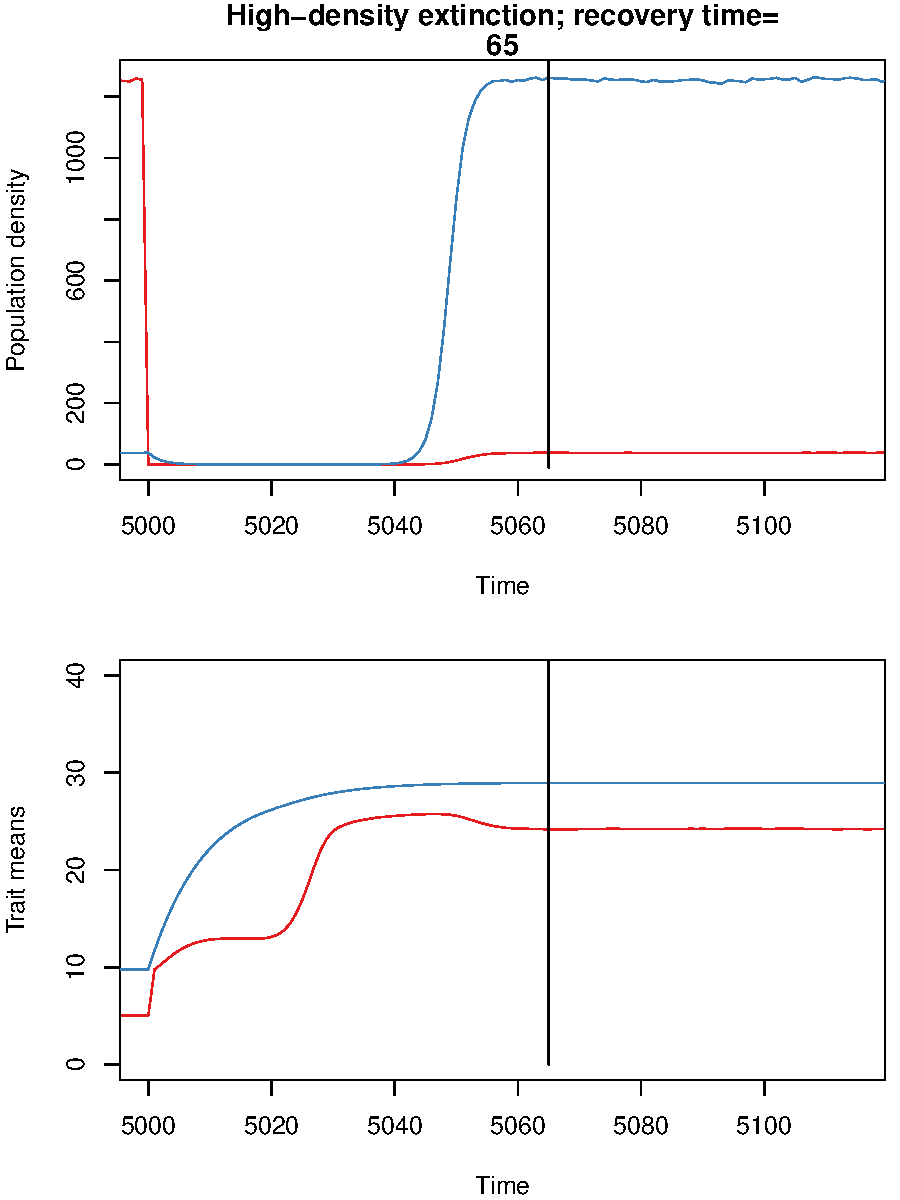
\includegraphics[width=0.35\textwidth]{fig_relax_inertia.pdf}
\caption{
Population inversion where increased differences in trait optima between sites $\Delta\theta$ corresponds to lower rates of straying $m$.
At low rates of straying $m=0.02$ ($\Delta\theta=24$), extinction of the dominant population leads to slower-than-expected recovery times because the subordinate population is isolated enough to evolve towards its own trait optimum. %until growth of the dominant population overwhelms this local selection.
In this case, $m$ is less than $m=0.034$ (denoted by the asterisk in figure \ref{extfig-fig:mtheta}), such that isolation allows the subordinate population to `run away' from the influence of the dominant population.
This leads to a switch in subordinate/dominant states for the two populations.
If $m$ is low but greater than $0.034$, isolation permits the subordinate population to `run away' from the influence of the dominant population, until it is overwhelmed by the recovering dominant population, and reverts back to its previous trait mean prior to disturbance.
} \label{fig:inertia}
\end{figure}


\begin{figure}
  \captionsetup{justification=raggedright,
singlelinecheck=false
}
  \centering
  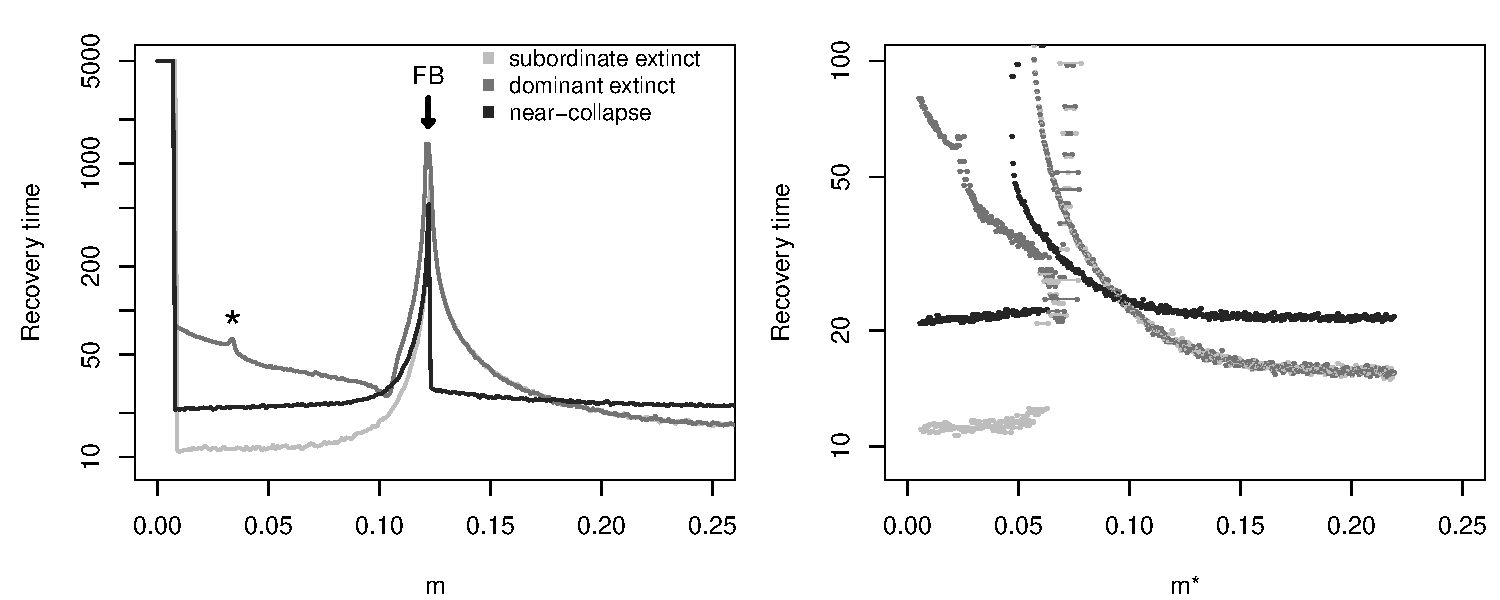
\includegraphics[width=0.8\textwidth]{fig_relax_mtheta.pdf}
  \caption{
  Recovery times for three disturbance types when the straying rate covaries with habitat heterogeneity as $m = 0.5(1 + \Delta\theta)^{-1}$ for constant (a) and density-dependent (b) straying rates.
  The cusp bifurcation is not as clear in (b) because $\Delta\theta$ is a function of the individual straying rate $m_0$, whereas the x-axis in (b) is the straying rate at the steady-state $m^*$.
  Despite this difference, the general behavior shown in (a) are the same in (b).
  } \label{fig:mthetamvm}
\end{figure}

\begin{figure}
  \captionsetup{justification=raggedright,
singlelinecheck=false
}
\centering
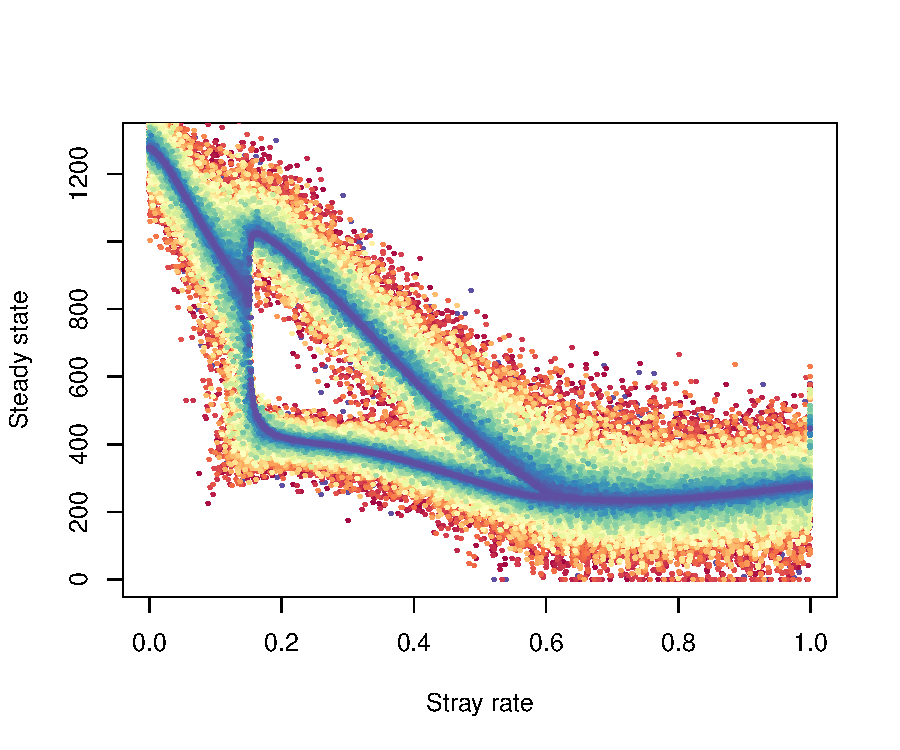
\includegraphics[width=0.35\textwidth]{fig_asymdensity.pdf}
\caption{
Steady-state densities of both populations as a function of $m$, where a cusp bifurcation indicates the emergence of alternative steady-states: one in a dominant state and one in a subordinate state.
Steady-states for populations with symmetrical values ($\alpha=0$) in the vital rates $r_{\rm max}$ and $\beta$ are shown with cool tones.
As the asymmetry among populations between sites increases ($\alpha>0$), their vital rates diverge, such that the maximal growth at sites 1 and 2 is now $r_{\rm max}(1)=r_{\rm max}(1+\tilde{rv}_1)$ and $r_{\rm max}(2)=r_{\rm max}(1+\tilde{rv}_2)$ where $rv_{1,2}$ are independently drawn from $\rm{Normal}(0,\alpha)$ and $r_{\rm max}=2$. 
Similarly the strength of density dependence is calculated at sites 1 and 2 as $\beta(1)=\beta(1+\tilde{rv}_1)$ and $\beta(2)=\beta(1+\tilde{rv}_2)$ where $\tilde{rv}_{1,2}$ are independently drawn from $\rm{Normal}(0,\alpha)$ and $\beta=0.001$.
Steady-states for populations with increasingly asymmetric values ($\alpha\rightarrow 0.1$) for vital rates $r_{\rm max}$ and $\beta$ are shown in warmer tones.
} \label{fig:symmetry}
\end{figure}


\begin{figure}
  \captionsetup{justification=raggedright,
singlelinecheck=false
}
\centering
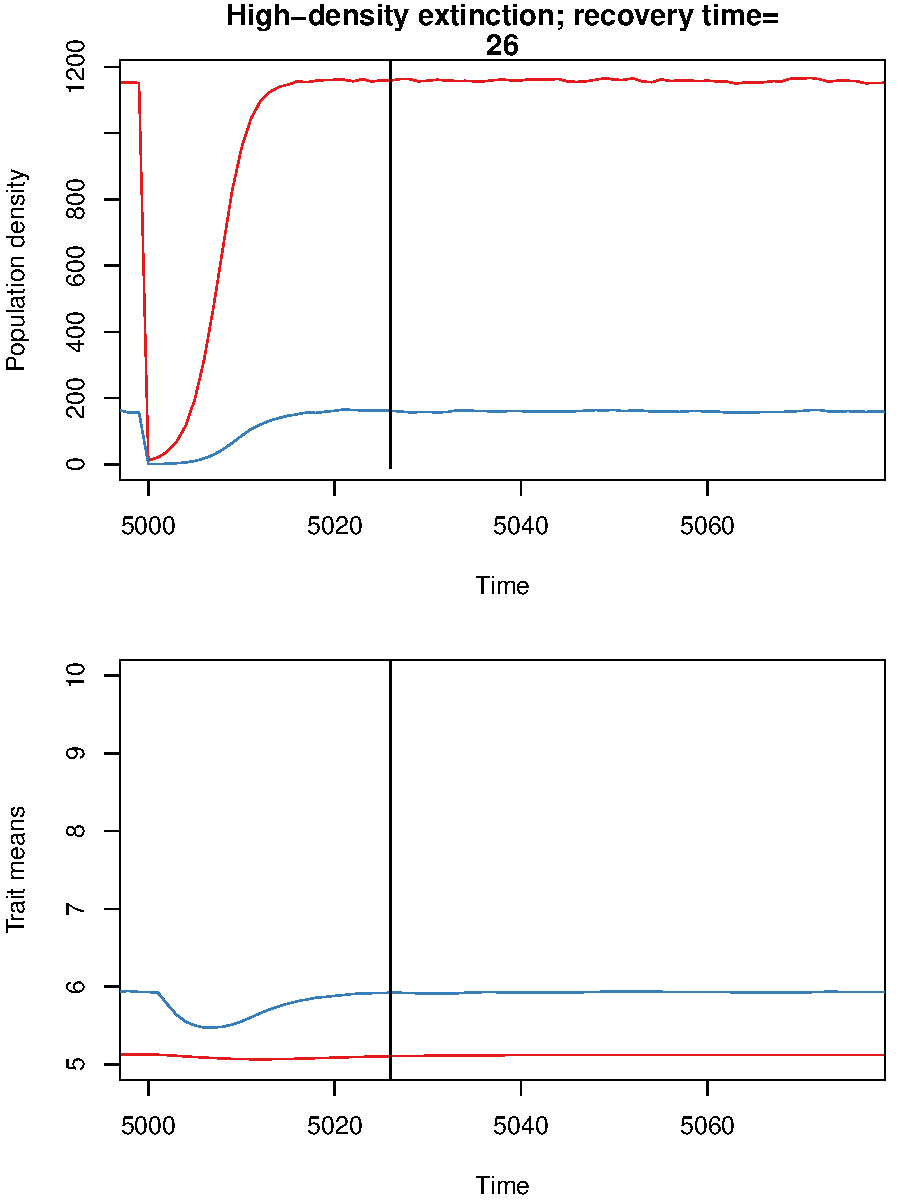
\includegraphics[width=0.35\textwidth]{fig_relax_both_lowh.pdf}
\caption{
Near collapse of both populations with a low straying rate $m=0.1$ and low trait heritability $h^2=0.2$ (see figure \ref{extfig-fig:relax}a).
Black line marks the calculated point of recovery post-perturbation.
Trait optima are $\theta_1 = 10$ (blue population trajectory) and $\theta_2 = 5$ (red population).
} \label{fig:relaxtraj_bothlh}
\end{figure}


\end{document}
